\section{Renormalization group on the Fibonacci chain}
\subsection{Dummy}

\begin{frame}{Renormalization group on the Fibonacci chain}
\(
\<{7cm}
Focused on the $E=0$ state\dots

{\centering
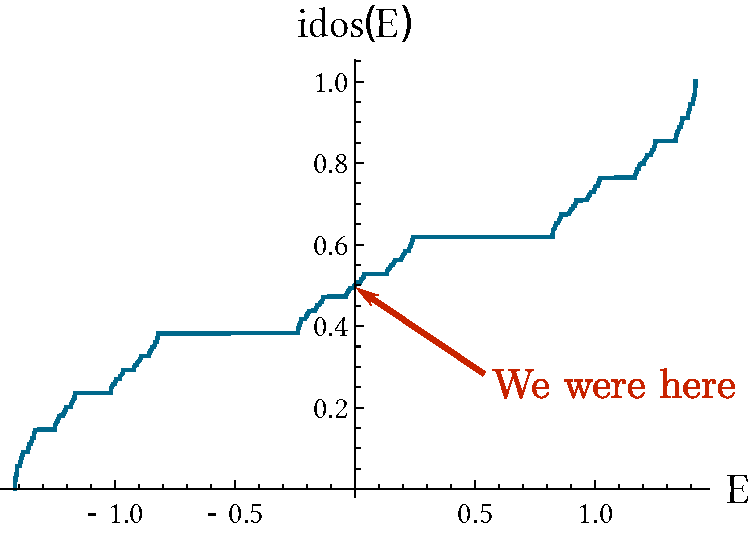
\includegraphics[width=.8\textwidth]{img/3_part2/idos_fibo}

{\ss Integrated density of states (IDoS) of the Fibonacci chain}

}

\dots what about the rest of the spectrum?
\>
\<{7cm}{Analytical results}
\begin{itemize}
	\item Gap labeling [Bellissard 86]
	\item Fractal dimensions of the spectrum
	\begin{itemize}
		\item $\rho = t_\A/t_\B \ll 1$: [Piéchon \etal{} 95]
		\item $\rho \sim 1$: [Rüdinger, Sire 96]
	\end{itemize}
	\item Fractal dimensions of the eigenstates, $\rho \ll 1$
	\begin{itemize}
		\item \textbf{leading order} 
		
		\textbf{[Thiem, Schreiber 12]}
		\item \textbf{higher order} 
		
		\textbf{[Macé \etal{} 16]}
	\end{itemize}
	\item exact description of the $E=0$ state
	
 	[Kohmoto \etal{} 87], [Macé \etal{} 17]
\end{itemize}
\>
\)
\end{frame}

\begin{frame}{Atoms and molecules}
Fibonacci chain in the limit $\rho = t_\A/t_\B = 0$:

{\centering
    	\begin{tikzpicture}[scale=.6]
    		\newcommand{\orig}{-1.5}
    		\newcommand{\trans}{1.5}
    		\newcommand{\vertspac}{-2.}    		
    		\newcommand{\rad}{2pt} % radii of the circles
    		\newcommand{\hh}{1.} % half height of the rectangle
    		\newcommand{\del}{.2} % distance between nodes and border of the rectangle

    		% set the style of the strong bonds
    		\tikzset{
    			strong/.style={
    				double,
    				double distance=\rad,
    				line width=0.5pt
    				}
    		}
    	
    		% initial chain
    	
    		% bonds 
			\draw[-] (\orig+\trans,0) -- (\orig+2*\trans,0) node [midway, above] {$t_\ca$};
			\draw[strong] (\orig+2*\trans,0) -- (\orig+3*\trans,0) node [midway, above] {$t_\cb$};	
			\draw[-] (\orig+3*\trans,0) -- (\orig+4*\trans,0) node [midway, above] {$t_\ca$};
			\draw[-] (\orig+4*\trans,0) -- (\orig+5*\trans,0) node [midway, above] {$t_\ca$};
			\draw[strong] (\orig+5*\trans,0) -- (\orig+6*\trans,0) node [midway, above] {$t_\cb$};
			\draw[-] (\orig+6*\trans,0) -- (\orig+7*\trans,0) node [midway, above] {$t_\ca$};
			\draw[strong] (\orig+7*\trans,0) -- (\orig+8*\trans,0) node [midway, above] {$t_\cb$};
			\draw[-] (\orig+8*\trans,0) -- (\orig+9*\trans,0) node [midway, above] {$t_\ca$};
    	
    	
    		% sites
		    \filldraw (\orig+1*\trans,0) circle (\rad) node [left] {\dots};% node [below] {6};
		    \filldraw (\orig+2*\trans,0) circle (\rad);% node [below] {3};
		    \filldraw (\orig+3*\trans,0) circle (\rad);% node [below] {8};
		    \filldraw (\orig+4*\trans,0) circle (\rad);% node [below] {5};
		    \filldraw (\orig+5*\trans,0) circle (\rad);% node [below] {2};
		    \filldraw (\orig+6*\trans,0) circle (\rad);% node [below] {7};
		    \filldraw (\orig+7*\trans,0) circle (\rad);% node [below] {4};
		    \filldraw (\orig+8*\trans,0) circle (\rad);% node [below] {1};
		    \filldraw (\orig+9*\trans,0) circle (\rad) node [right] {\dots};
		      
% draw a rectangle around a molecule
\draw [rounded corners, color=comp] (\orig+2*\trans-\del,-\hh) -- (\orig+3*\trans+\del,-\hh) node [midway, below] {molecule} -- (\orig+3*\trans+\del,+\hh) -- (\orig+2*\trans-\del,+\hh) -- cycle;

% draw a rectangle around an atom
\draw [rounded corners, color=BostonBlue] (\orig+4*\trans-\del,-\hh) -- (\orig+4*\trans+\del,-\hh) node [midway, below] {atom} -- (\orig+4*\trans+\del,+\hh) -- (\orig+4*\trans-\del,+\hh) -- cycle;

% draw a rectangle around a molecule
\draw [rounded corners, color=comp] (\orig+5*\trans-\del,-\hh) -- (\orig+6*\trans+\del,-\hh) node [midway, below] {molecule} -- (\orig+6*\trans+\del,+\hh) -- (\orig+5*\trans-\del,+\hh) -- cycle;

% draw a rectangle around a molecule
\draw [rounded corners, color=comp] (\orig+7*\trans-\del,-\hh) -- (\orig+8*\trans+\del,-\hh) node [midway, below] {molecule} -- (\orig+8*\trans+\del,+\hh) -- (\orig+7*\trans-\del,+\hh) -- cycle;
		\end{tikzpicture}


}

$\to$ collection of decoupled atoms and diatomic molecules

$\rho \neq 0,~\rho \ll 1$ $\to$ lifted degeneracy, atomic and molecular energy clusters:

{\centering
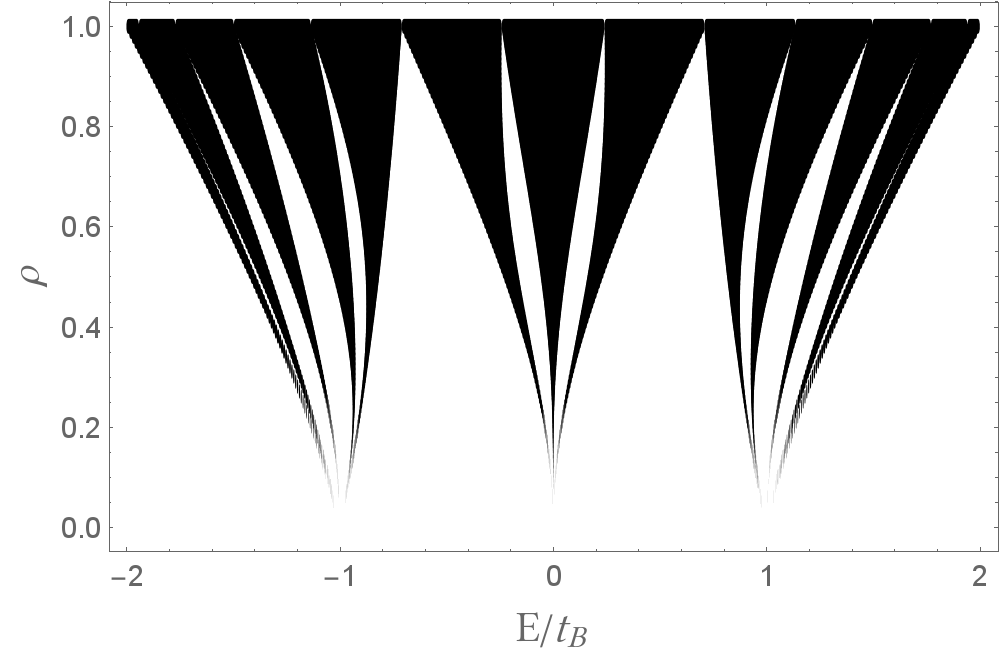
\includegraphics[width=.4\textwidth]{img/3_part2/fibonacci_spectra_varying_rho}

}

\end{frame}

\begin{frame}{Renormalization}
Substitution rule: $C_{l+1} = \sub(C_l)$ $\implies$ renormalization [Niu, Nori 86, Kalugin \etal{} 86]
	\begin{itemize}
	\item Atomic RG step (decimation of molecules) 
	
	{\centering
	\documentclass[talk.tex]{subfiles}
\begin{document}


    	\begin{tikzpicture}[scale=.7]
    		\newcommand{\orig}{-1.5}
    		\newcommand{\trans}{1.5}
    		\newcommand{\vertspac}{-2.}
    		\newcommand{\vertsize}{0} % vertical spand of the rectangles
    		\newcommand{\del}{.2}
    		\newcommand{\rad}{2pt} % radii of the circles
    	
    		% set the style of the strong bonds
    		\tikzset{
    			strong/.style={
    				double,
    				double distance=\rad,
    				line width=0.5pt
    				}
    		}
    		
    		% initial chain
    	
    		% bonds 
        	\draw[-] (\orig, 0)  node [left] {}  -- (\orig+\trans, 0)  node [midway, above] {$t_w$};
			\draw[strong] (\orig+\trans,0) -- (\orig+2*\trans,0)  node [midway, above] {$t_s$};
			\draw[-] (\orig+2*\trans,0) -- (\orig+3*\trans,0) node [midway, above] {$t_w$};	
			\draw[strong] (\orig+3*\trans,0) -- (\orig+4*\trans,0) node [midway, above] {$t_s$};
			\draw[-] (\orig+4*\trans,0) -- (\orig+5*\trans,0) node [midway, above] {$t_w$};
			\draw[-] (\orig+5*\trans,0) -- (\orig+6*\trans,0) node [midway, above] {$t_w$};
			\draw[strong] (\orig+6*\trans,0) -- (\orig+7*\trans,0) node [midway, above] {$t_s$};
			\draw[-] (\orig+7*\trans,0) -- (\orig+8*\trans,0) node [midway, above] {$t_w$};
    	
    		% sites
			\foreach \x in {0,...,7}
		      \filldraw (\orig+\x*\trans,0) circle (\rad); % node [below] {$\ket{\x}$};
		    % last site with chain step attached
		    \filldraw (\orig+8*\trans,0) circle (\rad) node [right] {~~~$n$};
		    
		    % rectangles around atoms
%		    \draw [rounded corners] (\orig-\vertsize,-\vertsize) rectangle (\orig+\vertsize,\vertsize);
%		    \draw [rounded corners] (\orig-\vertsize+5*\trans,-\vertsize) rectangle (\orig+\vertsize+5*\trans,\vertsize);
%		    \draw [rounded corners] (\orig-\vertsize+8*\trans,-\vertsize) rectangle (\orig+\vertsize+8*\trans,\vertsize);
		    
		    % arrows below rectangles
		    \draw [->] (\orig,-\vertsize-\del) -- (\orig,\vertspac+\del);
		    \draw [->] (\orig+5*\trans,-\vertsize-\del) -- (\orig+5*\trans,\vertspac+\del);
		    \draw [->] (\orig+8*\trans,-\vertsize-\del) -- (\orig+8*\trans,\vertspac+\del);
		      
		    % atomic chain
		    
        	\draw[-] (\orig, \vertspac)  node [left] {}  -- (\orig+5*\trans, \vertspac)  node [midway, above] {$\zb t_w$};
			\draw[strong] (\orig+5*\trans,\vertspac) -- (\orig+8*\trans,\vertspac) node [midway, above] {$\zb t_s$};
			
			\filldraw (\orig,\vertspac) circle (\rad); % node [below] {$\ket{\x}$};
			\filldraw (\orig+5*\trans,\vertspac) circle (\rad); % node [below] {$\ket{\x}$};
			\filldraw (\orig+8*\trans,\vertspac) circle (\rad) node [right] {~~~$n-3$};
		\end{tikzpicture}

\end{document}
	}
	
	\item Molecular RG step (decimation of atoms) 
	
	{\centering
	\documentclass[../fractal_dimensions_quasicrystals.tex]{subfiles}
\begin{document}


    	\begin{tikzpicture}[scale=.7]
    		\newcommand{\orig}{-1.5}
    		\newcommand{\trans}{1.5}
    		\newcommand{\vertspac}{-2.}
    		\newcommand{\vertsize}{0} % vertical span of the rectangles
    		\newcommand{\del}{.2}
    		\newcommand{\rad}{2pt} % radii of the circles

    		
    		% set the style of the strong bonds
    		\tikzset{
    			strong/.style={
    				double,
    				double distance=\rad,
    				line width=0.5pt
    				}
    		}
    	
    		% initial chain
    	
    		% bonds 
        	\draw[-] (\orig, 0)  node [left] {}  -- (\orig+\trans, 0) node [midway, above] {$t_w$};
			\draw[strong] (\orig+\trans,0) -- (\orig+2*\trans,0) node [midway, above] {$t_s$};
			\draw[-] (\orig+2*\trans,0) -- (\orig+3*\trans,0) node [midway, above] {$t_w$};	
			\draw[strong] (\orig+3*\trans,0) -- (\orig+4*\trans,0) node [midway, above] {$t_s$};
			\draw[-] (\orig+4*\trans,0) -- (\orig+5*\trans,0) node [midway, above] {$t_w$};
			\draw[-] (\orig+5*\trans,0) -- (\orig+6*\trans,0) node [midway, above] {$t_w$};
			\draw[strong] (\orig+6*\trans,0) -- (\orig+7*\trans,0) node [midway, above] {$t_s$};
			\draw[-] (\orig+7*\trans,0) -- (\orig+8*\trans,0) node [midway, above] {$t_w$};
    	
    		% sites
			\foreach \x in {0,...,8}
		      \filldraw (\orig+\x*\trans,0) circle (\rad); % node [below] {$\ket{\x}$};
		      
		    % rectangles around molecules
%		    \draw [rounded corners] (\orig +\trans-\del,-\vertsize) rectangle (\orig+2*\trans+\del,\vertsize);
%		    \draw [rounded corners] (\orig +3*\trans-\del,-\vertsize) rectangle (\orig+4*\trans+\del,\vertsize);
%		    \draw [rounded corners] (\orig +6*\trans-\del,-\vertsize) rectangle (\orig+7*\trans+\del,\vertsize);
		    
		    % arrows below rectangles
		    \draw [->] (\orig+1.5*\trans,-\vertsize-\del) -- (\orig+1.5*\trans,\vertspac+\del);
		    \draw [->] (\orig+3.5*\trans,-\vertsize-\del) -- (\orig+3.5*\trans,\vertspac+\del);
		    \draw [->] (\orig+6.5*\trans,-\vertsize-\del) -- (\orig+6.5*\trans,\vertspac+\del);
		      
			% molecular chains
			
			\foreach \x in {1}
			{
				\draw[-] (\orig, \x*\vertspac) node [left] {} -- (\orig+1.5*\trans, \x*\vertspac) node [midway, above] {$t_w'$};
				\draw[strong] (\orig+1.5*\trans, \x*\vertspac) -- (\orig+3.5*\trans, \x*\vertspac) node [midway, above] {$t_s'$};
				\draw[-] (\orig+3.5*\trans, \x*\vertspac) -- (\orig+6.5*\trans, \x*\vertspac) node [midway, above] {$t_w'$};
				\draw[strong] (\orig+6.5*\trans, \x*\vertspac) -- (\orig+8*\trans, \x*\vertspac) node [midway, above] {$t_s'$};
				
				\filldraw (\orig,\x*\vertspac) circle (\rad);
				\filldraw (\orig+1.5*\trans,\x*\vertspac) circle (\rad);
				\filldraw (\orig+3.5*\trans,\x*\vertspac) circle (\rad);
				\filldraw (\orig+6.5*\trans,\x*\vertspac) circle (\rad);
				\filldraw (\orig+8*\trans,\x*\vertspac) circle (\rad);
			}
		\end{tikzpicture}

\end{document}
	}
	
	\end{itemize}

	\flushleft{In the limit $\rho \ll 1$, $z= \rho/2$, $\zb = \rho^2$}
\end{frame}

\begin{frame}{RG construction \& renormalization paths}
 \[ H_l = \underbrace{\left( z H_{l-2} - t_s \right)}_{\text{\textcolor{BostonBlue}{bonding }levels}} + \underbrace{\left( \zb H_{l-3} \right)}_{\text{\textcolor{comp}{atomic} levels}} + \underbrace{\left( z H_{l-2} + t_s \right)}_{\text{\textcolor{BostonBlue}{antibonding} levels}} + \mathcal{O}(\rho^4)\]
	$\rightarrow$ recursive construction of the spectrum [Piéchon \etal{} 95]
	
	\begin{columns}
	\begin{column}{6cm}
	\centering
	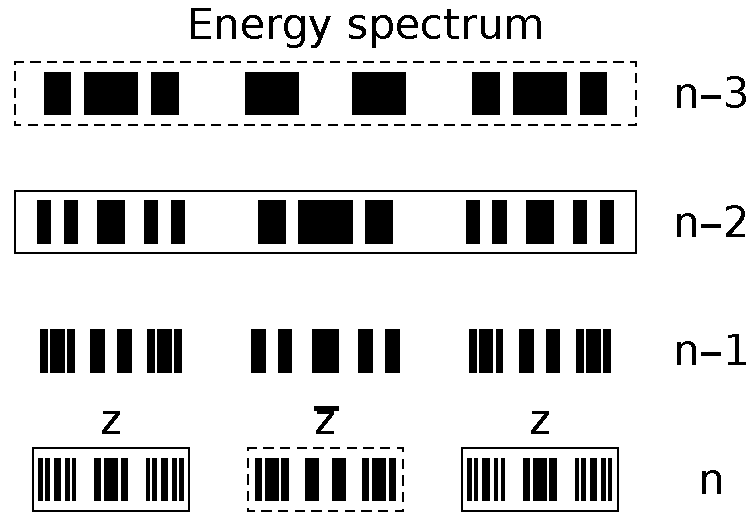
\includegraphics[scale=.4]{img/3_part2/recursive_construction_spectrum.pdf}
	\end{column}
	\begin{column}{6cm}
	Eigenstate $\leftrightarrow$ renormalization path:
	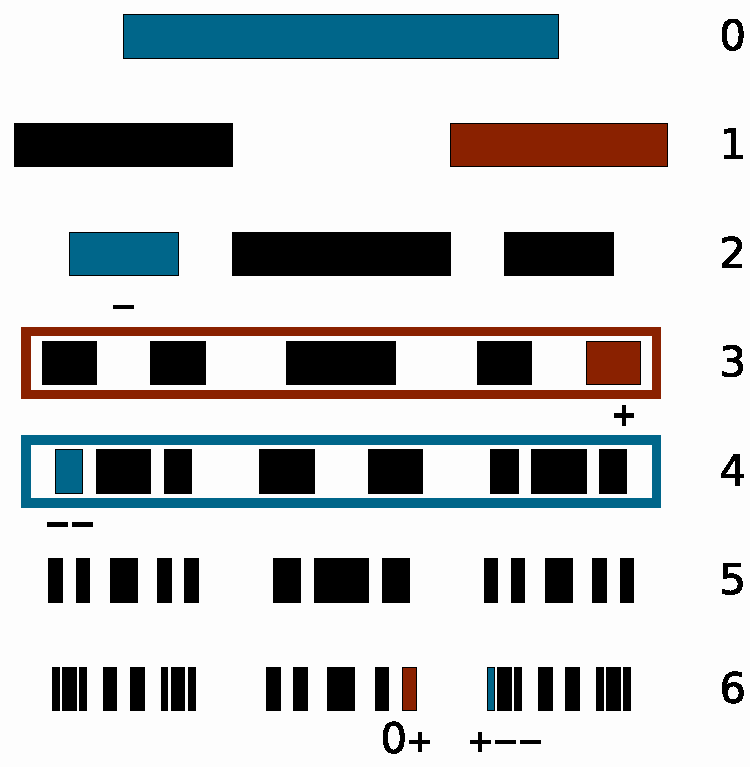
\includegraphics[scale=.3]{img/3_part2/renormalization_paths_spectrum.pdf}
	\end{column}
	\end{columns}
\end{frame}

\begin{frame}{RG for the eigenstates}
Cut-and-project $\to$ internal space $\to$ sites classified by local environment

{\centering	
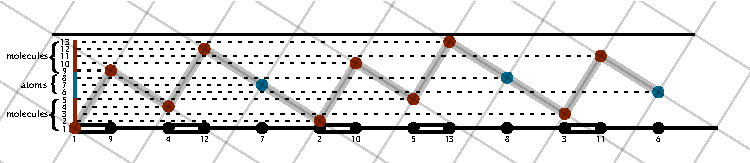
\includegraphics[width=.75\textwidth]{img/3_part2/cut_and_project}
	
}

Conumbering: numbering sites in internal space [Mosseri 88], [Mosseri, Sire 90].

\(
\<{5cm}
\centering
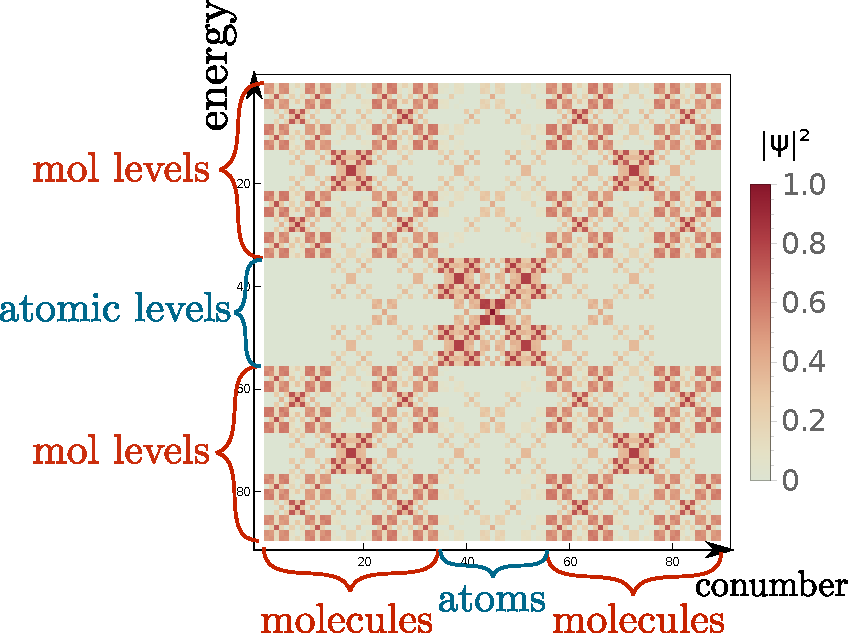
\includegraphics[width=.8\textwidth]{img/3_part2/ldos_reordered}

{\ss Fractal electronic density}
\>
\<{5cm}
\centering
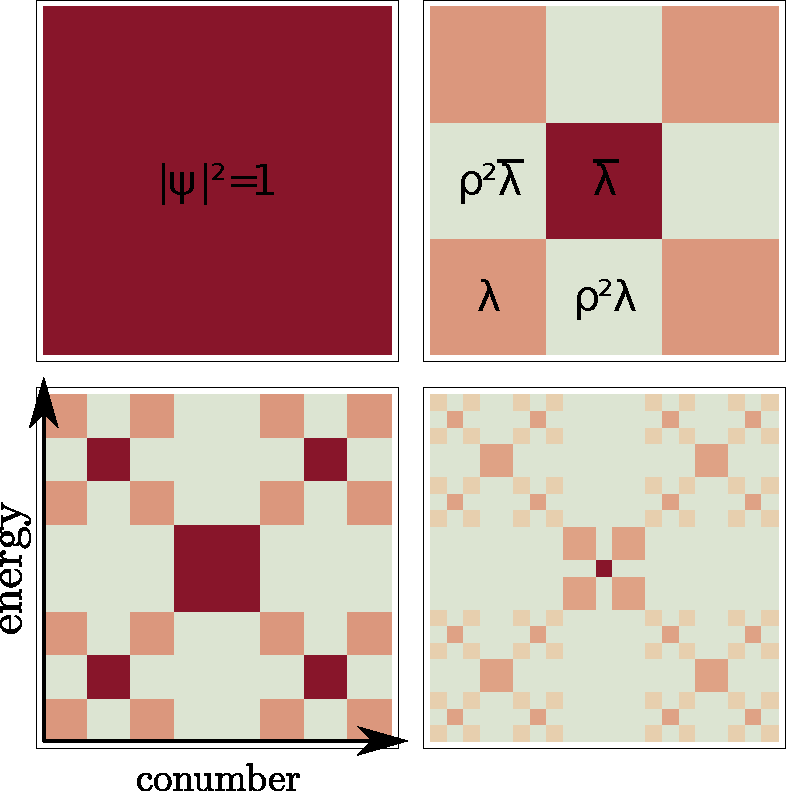
\includegraphics[width=.6\textwidth]{img/3_part2/recursion_idos}

{\ss Electronic density at different RG steps}
\>
\<{5cm}
Renormalization factors:

\textcolor{BostonBlue}{atomic} levels:

$|\psi_m^{(l)}(E)|^2 = \textcolor{BostonBlue}{\lb} |\psi_{m'}^{(l-3)}(E')|^2$

\textcolor{comp}{molecular} levels:

$|\psi_m^{(l)}(E)|^2 = \textcolor{comp}{\lambda} |\psi_{m'}^{(l-2)}(E')|^2$
\>
\)
\end{frame}

%\begin{frame}{Perturbative RG for the wavefunctions}
%Substitution rule: $C_{l+1} = \sub(C_l)$ $\implies$ real space renormalization [Niu, Nori 86, Kalugin \etal{} 86, Macé \etal{} 16]
%	\begin{itemize}
%
%		\item Atomic RG (decimation of the molecules)
%			\begin{columns}
%			\begin{column}{9cm}
%				%\documentclass[talk.tex]{subfiles}
%\begin{document}


    	\begin{tikzpicture}[scale=.6]
    		\newcommand{\orig}{-1.5}
    		\newcommand{\trans}{1.5}
    		\newcommand{\vertspac}{-2.}
    		\newcommand{\del}{.2}
    		\newcommand{\rad}{2pt} % radii of the circles
    	
    		% set the style of the strong bonds
    		\tikzset{
    			strong/.style={
    				double,
    				double distance=\rad,
    				line width=0.5pt
    				}
    		}
    		
    		% initial chain
    	
    		% bonds 
        	\draw[-] (\orig, 0)  node [left] {}  -- (\orig+\trans, 0);%  node [midway, above] {$t_w$};
			\draw[strong] (\orig+\trans,0) -- (\orig+2*\trans,0);%  node [midway, above] {$t_s$};
			\draw[-] (\orig+2*\trans,0) -- (\orig+3*\trans,0);% node [midway, above] {$t_w$};	
			\draw[strong] (\orig+3*\trans,0) -- (\orig+4*\trans,0);% node [midway, above] {$t_s$};
			\draw[-] (\orig+4*\trans,0) -- (\orig+5*\trans,0);% node [midway, above] {$t_w$};
			\draw[-] (\orig+5*\trans,0) -- (\orig+6*\trans,0);% node [midway, above] {$t_w$};
			\draw[strong] (\orig+6*\trans,0) -- (\orig+7*\trans,0);% node [midway, above] {$t_s$};
			\draw[-] (\orig+7*\trans,0) -- (\orig+8*\trans,0);% node [midway, above] {$t_w$};
    	
    		% sites
			\foreach \x in {0,...,7}
		      \filldraw (\orig+\x*\trans,0) circle (\rad); % node [below] {$\ket{\x}$};
		     \filldraw (\orig+8*\trans,0) circle(\rad) node [right] {~~~$C_l$};
		      
		    \filldraw (\orig+5*\trans,0) circle (0) node [shift={(-0.4,0.3)}] {$|\psi_m|$};
		    
		    % vertical arrows
		    \draw [->] (\orig,-\del) -- (\orig,\vertspac+\del) node [midway, right] {$\lb$};
		    \draw [->] (\orig+5*\trans,-\del) -- (\orig+5*\trans,\vertspac+\del) node [midway, right] {$\lb$};
		    \draw [->] (\orig+8*\trans,-\del) -- (\orig+8*\trans,\vertspac+\del) node [midway, right] {$\lb$};
		    
		    % horizontal arrows
%			\path [->] (\orig+5*\trans,+\del)  edge [bend left=-90] (\orig+3.5*\trans,+\del);
%			\path [->] (\orig+5*\trans,+\del)  edge [bend left=90] (\orig+6.5*\trans,+\del);
%			\path [->] (\orig+5*\trans,+\del)  edge [bend left=-90] (\orig+1.5*\trans,+\del);
		      
		    % atomic chain
		    
        	\draw[-] (\orig, \vertspac)  node [left] {}  -- (\orig+5*\trans, \vertspac);%  node [midway, above] {$t_w'$};
			\draw[strong] (\orig+5*\trans,\vertspac) -- (\orig+8*\trans,\vertspac);% node [midway, above] {$t_s'$};
			
			\filldraw (\orig,\vertspac) circle (\rad); % node [below] {$\ket{\x}$};
			\filldraw (\orig+5*\trans,\vertspac) circle (\rad) node [shift={(-0.7,0.3)}] {$\sqrt{\lb} |\psi_{m}|$};
			\filldraw (\orig+8*\trans,\vertspac) circle (\rad)node [right] {~~~$C_{l-3}$};
		\end{tikzpicture}

%\end{document}
%			\end{column}
%			\begin{column}{2cm}
%			\[ \lb \simop{\rho \ll 1} \frac{1}{1+2\rho^2}
%			\]
%			\end{column}
%			\end{columns}
%		\item Molecular RG (decimation of the atoms)
%			\begin{columns}
%			\begin{column}{9cm}
%				\documentclass[talk.tex]{subfiles}
\begin{document}


    	\begin{tikzpicture}[scale=.6]
    		\newcommand{\orig}{-1.5}
    		\newcommand{\trans}{1.5}
    		\newcommand{\vertspac}{-2.}
    		\newcommand{\vertsize}{0} % vertical span of the rectangles
    		\newcommand{\del}{.2}
    		\newcommand{\rad}{2pt} % radii of the circles

    		
    		% set the style of the strong bonds
    		\tikzset{
    			strong/.style={
    				double,
    				double distance=\rad,
    				line width=0.5pt
    				}
    		}
    	
    		% initial chain
    	
    		% bonds 
        	\draw[-] (\orig, 0)  node [left] {}  -- (\orig+\trans, 0);
			\draw[strong] (\orig+\trans,0) -- (\orig+2*\trans,0);
			\draw[-] (\orig+2*\trans,0) -- (\orig+3*\trans,0);	
			\draw[strong] (\orig+3*\trans,0) -- (\orig+4*\trans,0);
			\draw[-] (\orig+4*\trans,0) -- (\orig+5*\trans,0);
			\draw[-] (\orig+5*\trans,0) -- (\orig+6*\trans,0);
			\draw[strong] (\orig+6*\trans,0) -- (\orig+7*\trans,0);
			\draw[-] (\orig+7*\trans,0) -- (\orig+8*\trans,0);
    	
    		% sites
			\foreach \x in {0,...,7}
		      \filldraw (\orig+\x*\trans,0) circle (\rad); % node [below] {$\ket{\x}$};
		     \filldraw (\orig+8*\trans,0) circle(\rad) node [right] {~~~$n$};
		     
		     \filldraw (\orig+3*\trans,0) circle (0) node [above] {$|\psi_i|$};
		    
		    % arrows below rectangles
		    \draw [->] (\orig+1.5*\trans,-\vertsize-\del) -- (\orig+1.5*\trans,\vertspac+\del) node [midway, right] {$\lambda$};
		    \draw [->] (\orig+3.5*\trans,-\vertsize-\del) -- (\orig+3.5*\trans,\vertspac+\del) node [midway, right] {$\lambda$};
		    \draw [->] (\orig+6.5*\trans,-\vertsize-\del) -- (\orig+6.5*\trans,\vertspac+\del) node [midway, right] {$\lambda$};
		      
			% molecular chains
			
				\draw[-] (\orig, \vertspac) node [left] {} -- (\orig+1.5*\trans, \vertspac);
				\draw[strong] (\orig+1.5*\trans,\vertspac) -- (\orig+3.5*\trans, \vertspac);
				\draw[-] (\orig+3.5*\trans, \vertspac) -- (\orig+6.5*\trans, \vertspac);
				\draw[strong] (\orig+6.5*\trans, \vertspac) -- (\orig+8*\trans, \vertspac);
				
				\filldraw (\orig,\vertspac) circle (\rad);
				\filldraw (\orig+1.5*\trans,\vertspac) circle (\rad);
				\filldraw (\orig+3.5*\trans,\vertspac) circle (\rad) node [shift={(-0.8,0.3)}] {$\sqrt{\lambda} |\psi_{i}|$};
				\filldraw (\orig+6.5*\trans,\vertspac) circle (\rad);
				\filldraw (\orig+8*\trans,\vertspac) circle (\rad) node [right] {~~~$n-2$};
			
		\end{tikzpicture}

\end{document}
%			\end{column}
%			\begin{column}{2cm}
%			\[ \lambda \simop{\rho \ll 1} \frac{1}{2+\rho^2}
%			\]
%			\end{column}
%			\end{columns}
%	\end{itemize}
%%\begin{align*}
%%		|\psi_m^{(l)}(E)|^2 &= \lb |\psi_{m'}^{(l-3)}(E')|^2 \text{~if $E$ is in the central cluster}\\
%%		|\psi_m^{(l)}(E)|^2 &= \lambda |\psi_{m'}^{(l-2)}(E')|^2 \text{~if }E\text{~is in the edge clusters}
%%\end{align*}
%\end{frame}

%Fractal dimensions of the eigenstates:
%\[
%d_q(x) = \frac{\log \Big[ \left( \frac{\lambda(\rho)^q}{\lambda(\rho^q)} \right)^x \left( \frac{\bar{\lambda}(\rho)^q}{\bar{\lambda}(\rho^q)} \right)^{(1-2x)/2} \Big]}{(q-1)\log \tau^{-1}}
%\]

\begin{frame}{Fractality of the eigenstates}
\(
\<{7cm}{Leading order [Thiem, Schreiber 12]}

$\lb = 1$

$\lambda = 1/2$
\>
\<{7cm}{Higher order [Macé \etal{} 16]}

$\lb = \frac{1}{1+2\rho^2}$

$\lambda = \frac{1}{2+\rho^2}$
\>
\)

\(
\<{7cm}

{\centering

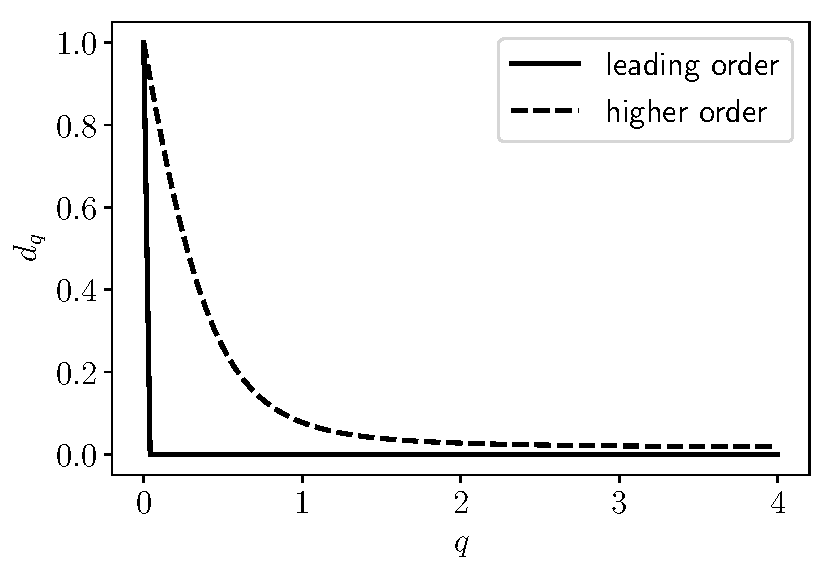
\includegraphics[width=.65\textwidth]{img/3_part2/fractal_dims_broccoli}

{\ss Fractal dimensions of the ``broccoli state'', $rho = 0.1$}

}

$\to$ higher order: captures multifractality
\>
\<{7cm}
\centering
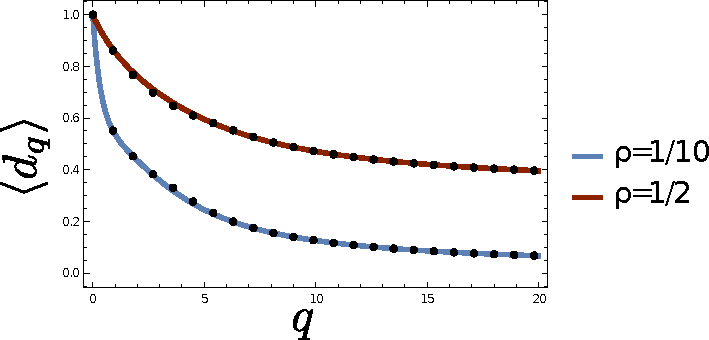
\includegraphics[width=.8\textwidth]{img/3_part2/average_wf_dimension}

{\ss Fractal dimensions averaged over all states: numerics \emph{vs} RG}

$\to$ higher order accurate for large $\rho$ 
\>
\)

\end{frame}

\begin{frame}{Conclusions}
Focus on the Fibonacci tight-binding chain, in the limit $\rho \ll 1$.
\begin{itemize}
	\item Substitution rule $\to$ \textbf{scale invariance} $\to$ renormalization group
	\item RG $\to$ eigenstates all \textbf{multifractal}
	\item Higher order in $\rho$: captures this multifractality
\end{itemize}
\end{frame}